% === T07 - Softcores, System On Chip y Diseño ===
% David Alejandro Gonzalez Marquez
% fokerman@gmail.com
% https://github.com/fokerman/fpgaSoftcoreProgrammingCourse

\RequirePackage[2020-02-02]{latexrelease}

\documentclass[aspectratio=169]{beamer}
\usepackage{../packages}

\newcommand{\na}{\cellcolor{naranjauca}}
\newcommand{\gm}{\cellcolor{gray!50}} 

\title{\Huge Softcores, System On Chip y Diseño}
\author{David Alejandro González Márquez}
\institute{Programación de softcores en FPGAs\\
Programa de Profesoras/es Visitantes\\
Departamento de computación\\
Universidad de Buenos Aires}


\date{}

\begin{document}

\begin{frame}[plain]
    \titlepage
    \begin{textblock}{110}(25,80)
    \begin{tcolorbox}[size=small,width=\textwidth,colback={gray!30},title={}]
    \begin{center}
     \scriptsize Clase disponible en: \url{https://github.com/fokerman/fpgaSoftcoreProgrammingCourse}
    \end{center}
    \end{tcolorbox}
    \end{textblock}
\end{frame}

\begin{frame}[t,fragile]
    \frametitle{Softcores, System On Chip y Diseño}
    Los procesadores diseñados o configurados especialmente para implementarse sobre un FPGA se denominan \textbf{Softcores}.\\
    \bigskip
    \pause
    Estos requieren soporte de acceso a memoria, memoria cache, periféricos y de sistemas de interconexión, construyendo lo que denominamos un \textbf{System On Chip}.\\
    \bigskip
    \pause
    Si el soporte es muy limitado, diseñado con un propósito específico y completamente embebido lo llamamos \textbf{Microcontrolador}.\\
    \bigskip
    \pause
    La interconexión por su parte requiere buses y control de estos, mediante alguna \textbf{interfaz de interconexión}.\\
    \bigskip
    \pause
    Adicionalmente no todo diseño es útil para cualquier problema.\\
    Es fundamental entender como combinar las capacidades del software con el hardware flexible para lograr un \textbf{Codiseño Hardware/Software} eficiente.\\
\end{frame}

\begin{frame}[t,fragile]
    \frametitle{Softcores}
    Existen diferentes implementaciones de \emph{Softcores} con distintas características y propiedades.\\
    \small \textcolor{verdeuca}{Estos pueden ser completamente configurables, o no, ser parte de una solución integrada a un SoC, ser completamente independientes o incluso limitarse a comportarse como un Microcontrolador.}\\
    \bigskip
    \normalsize
    Algunos ejemplos,
    \begin{itemize}
        \item PicoBlaze
        \item MicroBlaze
        \item LEONN3
        \item Nios II
        \item PULPino
        \item Rocket
        \item BOOM
    \end{itemize}
    \bigskip
    \textcolor{verdeuca}{Vamos a recorrer las características de agunos procesadores, SoC o MCU seleccionados.}
\end{frame}

\begin{frame}[t,fragile]
    \frametitle{Softcores - PicoBlaze}
    \begin{textblock}{140}(10,12) \footnotesize
    Microcontrolador de 16 bits desarrollado por Xilinx, con 1KB de memoria de instrucciones, 64 bytes de RAM, 256 puertos de entrada salida y pila de 31 posiciones. Bajo licencia BSD.\\
    \textcolor{verdeuca}{Todas las instrucciones demoran 2 ciclos (predecible), e interrupciones de respuesta rápida en 5 ciclos.}\\
    Optimizado para FPGAs, requiriendo solo 96 celdas según documentación.
    \end{textblock}
    \begin{textblock}{140}(10,28)
    \begin{center}
    \includegraphics[scale=0.7]{img/picoblaze.pdf}
    \end{center}
    \end{textblock}
\end{frame}

\begin{frame}[t,fragile]
    \frametitle{Softcores - MicroBlaze}
    \begin{textblock}{50}(10,12) \footnotesize
    Procesador de 32 bits completamente configurable, con soporte para todo tipo de conexiones e interfaces.\\
    \bigskip
    Integrado a las herramientas de Xilinx para su uso dentro de FPGAs del fabricante.\\
    \bigskip
    Soporta gran cantidad de bibliotecas de código. Es de código cerrado.
    \end{textblock}
    \begin{textblock}{10}(60,15)
    \includegraphics[scale=0.6]{img/microblaze_core.pdf}
    \end{textblock}
    
\end{frame}
    
\begin{frame}[t,fragile]
    \frametitle{Softcores - LEON3}
    \begin{textblock}{70}(10,15) \footnotesize
    Procesador de 32 bits basado en la arquitectura\\
    SPARC V8 desarrollado por Aeroflex Gaisler.\\
    \bigskip
    Completamente configurable, soportando hasta 16 cores implementados como \emph{asymmetric multiprocessing} (AMP) o \emph{synchronous multiprocessing} (SMP).
    \begin{center}
    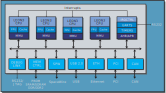
\includegraphics[scale=0.35]{img/leon3_system.pdf}
    \end{center}
    \end{textblock}
    \begin{textblock}{70}(80,10)
    \footnotesize Todo el código disponible bajo licencia GNU GPL para evaluación, investigación o fines educativos.\\
    \vspace{0.2cm}
    \includegraphics[scale=0.65]{imgBmp/BLOCK_LEON3.jpg}\\
    \end{textblock}
    \begin{textblock}{140}(10,78) \footnotesize
    \url{https://www.gaisler.com/index.php/products/processors/leon3}
    \end{textblock}
\end{frame}
    
\begin{frame}[t,fragile]
    \frametitle{Softcores - Nios II}
    \begin{textblock}{55}(10,12) \footnotesize
    Procesador de 32 bits desarrollado por Altera, actualmente Intel.\\
    \bigskip
    Diseñado como procesador embebido de propósito general, posee un pipeline de 5 etapas In-Order y un predictor de saltos estático.\\
    \bigskip
    Soportado dentro de las herramientas de Altera, con diferentes configuraciones.\\
    \bigskip
    Es de código cerrado.
    \end{textblock}
    \begin{textblock}{14}(70,8)
    \includegraphics[scale=0.7]{img/Nios.pdf}
    \end{textblock}
    \begin{textblock}{70}(10,75) \footnotesize
    \url{https://www.intel.com/content/www/us/en/products/details/fpga/nios-processor.html}
    \end{textblock}
\end{frame}
    
\begin{frame}[t,fragile]
    \frametitle{Softcores - PULPino}
    \begin{textblock}{55}(10,12) \footnotesize
    Procesador de 32 bits basado en RISC-V desarrollado por ETH Zurich.\\
    \bigskip
    Su implementación es In-Orden single-issue con un pipeline de 4 etapas.\\
    \bigskip
    \textcolor{gray}{Configurable y diseñado para muy bajo consumo y muy poca área.\\
    Soporta extensiones para punto flotante de precisión simple.}\\
    \bigskip
    Distribuido bajo licencia Apache 2.0. y codificado en System Verilog.
    \end{textblock}
    \begin{textblock}{55}(70,5) \includegraphics[scale=0.13]{imgBmp/PULPino_core.png} \end{textblock}
    \begin{textblock}{55}(75,37) \includegraphics[scale=0.13]{imgBmp/PULPino_system.png} \end{textblock}
    \begin{textblock}{70}(10,75) \footnotesize
    \url{https://github.com/pulp-platform/pulpino}
    \end{textblock}
% A near-threshold RISC-V core with DSP extensions for scalable IoT Endpoint Devices
% arXiv:1608.08376v1 [cs.AR] 30 Aug 2016
% Michael Gautschi, Student Member, IEEE,
% Pasquale Davide Schiavone, Student Member, IEEE, Andreas Traber, Igor Loi, Member, IEEE, Antonio Pullini, Student
% Member, IEEE, Davide Rossi, Member, IEEE, Eric Flamand, Frank K. Gürkaynak, and Luca Benini, Fellow, IEEE
\end{frame}
    
\begin{frame}[t,fragile]
    \frametitle{Softcores - Rocket}
    \begin{textblock}{68}(10,12) \footnotesize
    Procesador desarrollado por Berkeley, actualmente mantenido por SiFive. \textcolor{verdeuca}{Empresa privada que comercializa soluciones basadas en este procesador.}\\
    \bigskip
    Es un procesador In-Order single-issue con un pipeline de 5 etapas.\\
    \begin{center}
     \includegraphics[scale=0.5]{img/Rocket_pipeline.pdf}
    \end{center}
    Junto con memorias cache para datos y código se construye un \emph{tile} que se utilza como procesador del Rocket Chip SoC.
    \textcolor{verdeuca}{Completamente codificado en Chisel.}
    \end{textblock}
    \begin{textblock}{55}(90,10) \includegraphics[scale=0.6]{img/Rocket_system.pdf} \end{textblock}
    \begin{textblock}{140}(10,78) \footnotesize
    \url{https://github.com/chipsalliance/rocket-chip}
    \end{textblock}
\end{frame}

\begin{frame}[t,fragile]
    \frametitle{Softcores - Boom}
    \begin{textblock}{70}(10,12) \footnotesize
    Procesador desarrollado por Berkeley basado en RISC-V.\\ Soporta hasta las extensiones RV64GC.\\
    \bigskip
    Su microarquitectura es Out-Of-Order, parametrizable y diseñada para alto rendimiento.\\
    \bigskip
    Creado el grupo de Arquitectura de Procesadores con objetivos de académicos y de investigación.\\
    \bigskip 
    La última versión BOOMv3 alcanza un rendimiento similar a procesadores comerciales equivalentes.\\
    \bigskip
    Esta codificado en Chisel y distribuido bajo licencias BSD.
    \end{textblock}
    \begin{textblock}{10}(90,0) \includegraphics[scale=0.32]{imgBmp/BOOM_uarch.png} \end{textblock}
    \begin{textblock}{140}(10,80) \footnotesize
    \url{https://github.com/riscv-boom/riscv-boom}
    \end{textblock}
\end{frame}

\begin{frame}[t,fragile]
    \frametitle{Interconexionado}
    \small
    Existen múltiples soluciones propietarias de buses y sistemas para la interconexión de dispositivos, ya sea on-chip o off-chip.
    \uncover<2->{
    \textcolor{verdeuca}{Sin embargo el más utilizado es AMBA (Advanced Microcontroller Bus Architecture), un protocolo abierto desarrollado por ARM.}\\
    }
    \bigskip
    \uncover<3->{
    Este protocolo especifica el mecanismo la interconexión on-chip para la comunicación y administración de bloques funcionales en un SoC.\\
    }
    \begin{itemize}
    \setlength\itemsep{0.02cm}
    \item[1996]<4-> \small Primera versión. Especificación de Advanced System Bus (ASB) y Advanced Peripheral Bus (APB).
    \item[1999]<4-> \small AMBA 2, se agrega High-performance Bus (AHB) que implementa transferencias en dos etapas.
    \item[2003]<5-> \small AMBA 3, incluye Advanced eXtensible Interface (AXI) para soluciones de mayor rendimiento y Advanced Trace Bus (ATB) como solución de debug on-chip.
    \item[2010]<5-> \small AMBA 4, se introducen las especificaciones de AXI4.
    \item[2010]<6-> \small Extensiones para coherencia en todo el sistema usando AMBA 4 AXI Coherency Extensions (ACE).
    \item[2013]<6-> \small AMBA 5, introducen el Coherent Hub Interface (CHI). Mejora los mecanismos de coherencia.
    \end{itemize}
    \uncover<6->{
    \scriptsize \url{https://www.arm.com/architecture/system-architectures/amba/amba-specifications}
    }
\end{frame}

\begin{frame}[t,fragile]
    \frametitle{Interconexionado - AMBA}
    Estos protocolos se comercializan mediante una familia de dispositivos sintetizables de propiedad intelectual (\emph{synthesizable intellectual property (IP) cores}).\\
    \vspace{0.2cm}
    \uncover<2->{\textcolor{verdeuca}{Productos licenciados por ARM que implementan buses digitales on-chip para mover y almacenar eficientemente información bajo la especificación de los protocolos AMBA.}\\}
    \begin{textblock}{10}(10,35) \uncover<2->{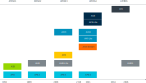
\includegraphics[scale=0.6]{img/AMBA_timeline.pdf}} \end{textblock}
    \begin{textblock}{40}(105,38) \small
     \uncover<3->{Muchos fabricantes utilizan los buses AMBA en diseños no ARM.\\}
     \bigskip
     \uncover<4->{\textcolor{verdeuca}{Xilinx implementa sus propios IP para utilizar protocolos AMBA dentro de sus FPGA.}\\}
     \bigskip
     \uncover<5->{\textcolor{naranjauca}{Actualmente es un estandar de facto}}
    \end{textblock}
\end{frame}

\begin{frame}[t,fragile]
    \frametitle{Interconexión - Protocolo AXI}  
    La especificación AXI define la interfaz que los bloques IP\\
    deben cumplir para la interconexión.\\
    \pause
    \bigskip
    En AXI, solo hay dos tipos de interfaces: \textbf{master} y \textbf{slave}.\\
    \textcolor{verdeuca}{Ambas interfaces son simétricas.}\\
    \pause
    \bigskip
    \textcolor{gray}{Todas las conexiones AXI se realizan entre interfaces\\
    maestras e interfaces esclavas.}\\
    \pause
    \bigskip
    Las interfaces de interconexión AXI contienen las mismas\\
    señales, lo que hace que la integración de diferentes IP\\
    sea relativamente simple.
    \begin{textblock}{10}(120,12) 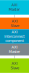
\includegraphics[scale=0.7]{img/AMBA_AXI_protocol_overview.pdf} \end{textblock}
\end{frame}

\begin{frame}[t,fragile]
    \frametitle{Interconexión - Protocolo AXI - Inter-connection architecture}
    \vspace{0.3cm}
    Ejemplo simplificado de un sistema SoC,\\
    que se compone de maestros, esclavos y\\
    la interconexión que conecta todo.\\
    \pause
    \bigskip
    \textcolor{gray}{Un procesador podría ser un ejemplo de\\
    maestro, y un controlador de memoria\\
    podría ser un ejemplo de esclavo.}\\
    \pause
    \bigskip
    \small
    AXI define las señales y la temporización de las conexiones punto a punto entre maestros y esclavos.\\
    Cuando están involucrados varios maestros y esclavos, se requiere una estructura de interconexión.\\
    \bigskip
    \textcolor{verdeuca}{El \emph{interconnect fabric} también implementa interfaces maestras y esclavas, donde se implementa el protocolo AXI.}
    \begin{textblock}{10}(80,12) 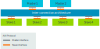
\includegraphics[scale=0.7]{img/AMBA_multi-master_system.pdf} \end{textblock}
\end{frame}

\begin{frame}[t,fragile]
    \frametitle{Interconexión - Protocolo AXI - Channels}
    \begin{textblock}{10}(90,12) 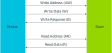
\includegraphics[scale=0.53]{img/AMBA_AXI_channels.pdf} \end{textblock}
    \begin{textblock}{80}(10,11)
    \small
    AXI define canales para la comunicación.\\
    \bigskip
    \uncover<2->{
    Operaciones de escritura:
    \begin{itemize}
    \item \footnotesize El maestro envía una dirección en el canal \textbf{Write\\
    Address (AW)} y transfiere datos en el canal \textbf{Write\\
    Data (W)} al esclavo.
    \item \footnotesize El esclavo escribe los datos recibidos en la dirección\\
    especificada. Una vez que el esclavo ha completado\\
    la operación de escritura, responde con un mensaje\\
    al maestro en el canal \textbf{Write Response (B)}.
    \end{itemize}
    }
    \uncover<3->{
    Operaciones de lectura:\\
    \begin{itemize}
    \item \footnotesize El maestro envía la dirección que desea leer en el canal\\
    \textbf{Read Address (AR)}.
    \item \footnotesize El esclavo envía los datos desde la dirección solicitada\\
    al maestro en el canal \textbf{Read Data (R)}.
    \end{itemize}
    }
    \end{textblock}
    \begin{textblock}{60}(90,46) \footnotesize 
    \uncover<4->{El esclavo también puede devolver un mensaje de error en el canal \textbf{Read Data (R)}.\\
    \textcolor{verdeuca}{Se produce un error si, por ejemplo, la dirección no es válida, o los datos están dañados, o el acceso no tiene el derecho permiso de seguridad.}\\
    }
    \bigskip
    \uncover<5->{
    Cada canal es \textbf{unidireccional}, por lo que se necesita un canal de respuesta de escritura independiente para pasar las respuestas de vuelta al maestro.
    }
    \end{textblock}
\end{frame}

% AXI MODOS
%     - stream
%     - Memory mapped

% Memory mapped (Channels)
% 
% AXI Slave
% AXI Master
% 
% 5 canales dependiendo de escrituras o lecturas
% 
% = Lecturas
% read data
% read address
% 
% = Escritura
% write address
% write data
% write response

% == Señales - write transaction
% awvalid ->
% awadds ->
% awready ->
% awlen ->
% awsize ->
% awid ->
% awcache --> sabe si es una cache!
% 
% Señales - write transaction - write data
% wvalid -> 
% wdata ->  
% wready -> 
% wlast -> 
% wstrb -> 
% 
% Señales - write transaction - write response
% bvalid -> 
% bready -> 
% bresp -> 
% bid -> 
% 
% == Señales - read transaction
% arvalid ->
% aradds ->
% arready ->
% arlen ->
% arsize ->
% arid ->
% arcache --> sabe si es una cache!
% 
% Señales - read transaction - write response
% rvalid ->
% rready ->
% rdata ->
% rlast ->
% rid -> 
% 
% Siempre tiene que responder!
% 
% Existen otras señales 
% 
% Low-power interface
% - Los dispositivos pueden cambiar entre modos de consumo.
% 
% Protection type
% - Identifican el nivel de seguridad de la transacción.
% 
% Quality of service of a transactions
% - Indican la prioridad de la transacción.
% 
% Region identifiers
% - Soporte para multiples regiones en un solo dispositivo esclavo.
% 
% User defined signals
% - Definidas por el usuario.

\begin{frame}[t,fragile]
    \frametitle{System On Chip}
    \begin{textblock}{140}(10,12) \small
    Un SoC combina componentes bajo un mismo bus.\\
    El procesador (típicamente RISC) que juega el rol\\ de conductor del SoC.\\
    \bigskip
    \uncover<2->{
    \textcolor{gray}{
    Otros componentes también son incluidos, memorias\\
    on-chip, interfaces de memoria off-chip, dispositivos\\
    dedicados, co-procesadores, e infraestructura de\\ comunicación entre componentes.\\}
    }
    \bigskip
    \uncover<3->{
    \textcolor{verdeuca}{El \textbf{dominio de la aplicación} afecta sustancialmente el tipo dispositivos, tamaño de la memoria\\ y la naturaleza de las comunicaciones on-chip.}\\
    }
    \bigskip
    \uncover<4->{
    Una configuración particular de todos estos elementos se denomina \textbf{plataforma}, especializada para un dominio de computo particular.
    }
    \end{textblock}
    \begin{textblock}{10}(86,7) 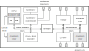
\includegraphics[scale=0.7]{img/Generic_SoC_C7F1.pdf} \end{textblock}
\end{frame}

\begin{frame}[t,fragile]
    \frametitle{System On Chip}
    La especialización de un SoC tiene las siguientes ventajas:\\
    \vspace{0.3cm}
    \begin{itemize}
    \setlength\itemsep{0.5cm}
    \item<1-> La \textbf{especialización} asegura que su eficiencia de procesamiento sea mayor en comparación con las soluciones de propósito general.\\
    \textcolor{gray}{Una mayor eficiencia de procesamiento significa un menor consumo de energía (mayor duración de la batería) o un mayor rendimiento absoluto.}
    \item<2-> La \textbf{flexibilidad} asegura que sea una solución reutilizable que funcione en múltiples aplicaciones.\\
    \textcolor{gray}{Como resultado, el costo por aplicación del diseño disminuye, las aplicaciones se pueden desarrollar más rápido y el SoC en sí mismo se vuelve más barato porque se puede fabricar para un mercado más grande.}
    \end{itemize}
\end{frame}

\begin{frame}[t,fragile]
    \frametitle{System On Chip}
    \begin{textblock}{10}(86,7) 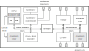
\includegraphics[scale=0.7]{img/Generic_SoC_C7F1.pdf} \end{textblock}
    La arquitectura de un SoC se puede analizar\\ en cuatro aspectos ortogonales:\\
    \begin{enumerate}
    \item Control
    \item Comunicación
    \item Computo
    \item Almacenamiento
    \end{enumerate}
    \vspace{0.2cm}
    \small
    \pause
    El rol de \textbf{control} lo toma el procesador, responsable de señales de control y recopilar el estado de los componentes.
    Puede contar o no con memoria de instrucciones local (o bien una cache).\\
    \vspace{0.2cm}
    \pause
    La \textbf{comunicación} se implementa usando buses a lo largo de todo el sistema. Donde cada componente responde a un determinado rango de memoria. Inclusive contando con DMAs.\\
    \vspace{0.2cm}
    \pause
    \textcolor{gray}{Es común dividir los buses en segmentos. Limitando la cantidad de componentes conectados a cada segmento de acuerdo con la necesidad de comunicación.}
\end{frame}

\begin{frame}[t,fragile]
    \frametitle{Interfaces con Hardware dedicado}
    \begin{textblock}{10}(86,1) 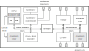
\includegraphics[scale=0.7]{img/Generic_SoC_C7F1.pdf} \end{textblock}
    \small
    En un SoC podemos integrar módulos de hardware\\
    personalizado.
    \uncover<2->{
    \textcolor{verdeuca}{Esto quiere decir una máquina\\
    digital dedicada descrita como un FSM o como\\
    una máquina microprogramada.\\}}
    \bigskip
    \uncover<3->{Se pueden distinguir tres enfoques:}
    \begin{itemize}
    \item<3-> Integrar un módulo de hardware personalizado como un \textbf{periférico} estándar en un bus del sistema.
    \textcolor{verdeuca}{El microprocesador se comunica con el módulo de hardware personalizado mediante accesos a memoria de lectura/escritura.}
    \item<4-> Conectar hardware personalizado a través de un \textbf{bus local} o una interfaz de coprocesador proporcionada por el microprocesador.
    \textcolor{verdeuca}{La comunicación entre el módulo y el microprocesador seguirá un protocolo dedicado, definido por el bus local o la interfaz del coprocesador.}
    \item<5-> Los microprocesadores también pueden proporcionar un medio para \textbf{integrar hardware personalizado} dentro del microprocesador.
    \textcolor{verdeuca}{Luego, el conjunto de instrucciones del microprocesador se amplía con nuevas instrucciones adicionales para controlar este hardware personalizado.}
    \end{itemize}
\end{frame}

\begin{frame}[t,fragile]
    \frametitle{Principios de diseño de Arquitecturas SoC}
    Si bien un SoC es un dispositivo muy específico para un dominio de aplicación.\\
    \textcolor{verdeuca}{Existen algunas máximas que se deben considerar en el diseño.}\\
    \bigskip
    A continuación se presentan cuatro principios de diseño que rigen la mayoría de las arquitecturas SoC.
    \bigskip
    \begin{enumerate}
    \setlength\itemsep{0.3cm}
    \item Procesamiento de datos heterogéneo y distribuido. %Heterogeneous and Distributed Data Processing
    \item Comunicaciones heterogéneas y distribuidas. %Heterogeneous and Distributed Communications
    \item Almacenamiento heterogéneo y distribuido. %Heterogeneous and Distributed Storage
    \item Control jerárquico. %Hierarchical Control
    \end{enumerate}
    \bigskip
    \textcolor{gray}{Vamos a ir describiendo cada una de las maximas.}
\end{frame}

\begin{frame}[t,fragile]
    \frametitle{Procesamiento de datos heterogéneo y distribuido}
    Un SoC puede contener múltiples unidades computacionales independientes (distribuidas).\\
    \textcolor{verdeuca}{Estas unidades pueden ser heterogéneas e incluir FSM, máquinas microprogramados o microprocesadores.\\}
    \bigskip
    \pause
    Se pueden distinguir tres formas de paralelismo de procesamiento de datos.
    \begin{enumerate}
    \item Paralelismo a \textbf{nivel de palabra}\\
    \textcolor{gray}{Permite el procesamiento paralelo de múltiples bits en una palabra.}
    \item Paralelismo a \textbf{nivel de operación}\\
    \textcolor{gray}{Permite ejecutar múltiples instrucciones simultáneamente.}
    \item Paralelismo a \textbf{nivel de tareas}\\
    \textcolor{gray}{Permite que múltiples hilos de control independientes se ejecuten de forma independiente.}
    \end{enumerate}
    \bigskip
    Solo un SoC admite el paralelismo a nivel de tarea.
\end{frame}

\begin{frame}[t,fragile]
    \frametitle{Comunicaciones heterogéneas y distribuidas}
    El bus central es un recurso crítico compartido por muchos componentes en un SoC.\\
    \bigskip
    \pause
    Para evitar que este recurso se convierta en un \textbf{cuello de botella} se divide el bus en varios \textbf{segmentos} utilizando \emph{bus bridges}.\\
    \textcolor{verdeuca}{El \emph{bus bridge} es un mecanismo para distribuir la comunicación en el chip.\\}
    \bigskip
    \pause
    Los requisitos de comunicación en el chip suelen ser variados, por lo tanto los mecanismos de interconexión de SoC también deberían ser heterogéneos.\\
    \vspace{0.2cm}
    \textcolor{gray}{Puede haber buses compartidos, conexiones punto a punto, conexiones en serie y conexiones en paralelo.\\}
    \bigskip
    \pause
    Las comunicaciones SoC heterogéneas y distribuidas permiten a un diseñador \textbf{explotar el ancho de banda de comunicación en el chip}.\\
\end{frame}

\begin{frame}[t,fragile]
    \frametitle{Almacenamiento heterogéneo y distribuido}
    En lugar de una sola memoria central, un SoC utilizará una colección de memorias dedicadas.\\
    \bigskip
    \begin{itemize}
    \setlength\itemsep{0.3cm}
    \item<2-> Los \textcolor{verdeuca}{procesadores} pueden contener memorias de instrucciones \textcolor{verdeuca}{locales} o utilizar \textcolor{verdeuca}{memorias caché} para mantener copias locales de datos e instrucciones.\\
    \item<3-> Los \textcolor{verdeuca}{coprocesadores} y otros componentes pueden utilizar \textcolor{verdeuca}{bancos de registros locales}.\\
    \item<4-> Los \textcolor{verdeuca}{aceleradores especializados} pueden usar memorias dedicadas para aplicaciones específicas, como almacenamiento en \textcolor{verdeuca}{buffers de bloques} o \textcolor{verdeuca}{un \emph{local scratchpad}}.\\
    \end{itemize}
    \bigskip
    \uncover<5->{Este almacenamiento se implementa con una colección de diferentes tecnologías de memoria.\\
    \vspace{0.2cm}
    \textbf{\textcolor{naranjauca}{Existen cinco categorías básicas almacenamiento basado en silicio.}}}
\end{frame}

\begin{frame}[fragile]
    \frametitle{Almacenamiento heterogéneo y distribuido}
    \small
    \begin{itemize}
    \item<1-> Los \textbf{registros} son el tipo de memoria más rápido disponible. \textcolor{verdeuca}{Residen más cerca de los elementos de computación de una arquitectura.}
    \item<2-> La \textbf{memoria dinámica de acceso aleatorio} (DRAM) proporciona almacenamiento económico a densidades muy altas. \textcolor{verdeuca}{A diferencia de los registros, las celdas DRAM utilizan una tecnología diferente y por lo tanto, son más complejas de interar en un solo chip.}
    \item<3-> La \textbf{memoria estática de acceso aleatorio} (SRAM) se utiliza cuando se requiere un almacenamiento rápido de lectura y escritura. \textcolor{verdeuca}{SRAM tiene menor densidad y mayor consumo de energía que DRAM. Facil de integrar, utiliza la misma tecnología que los SoC.}
    \item<4-> La \textbf{memoria no volátil de solo lectura} (NVROM) se usa para aplicaciones que solo requieren acceso de lectura en una memoria. \textcolor{verdeuca}{Por ejemplo para almacenar las instrucciones de un programa. Las memorias no volátiles tienen una densidad más alta que la SRAM.}
    \item<5-> La \textbf{memoria de acceso aleatorio no volátil} (NVRAM) se usa para aplicaciones que necesitan memorias de lectura y escritura que no pierden datos cuando se desconecta la alimentación. \textcolor{verdeuca}{La velocidad de lectura y escritura en una NVRAM puede ser asimétrica.}
    \end{itemize}
\end{frame}

\begin{frame}[t,fragile]
    \frametitle{Control jerárquico}
    \small
    Una jerarquía de control significa que todo el SoC opera como \textcolor{naranjauca}{\textbf{una sola entidad lógica}.}\\
    \textcolor{verdeuca}{Esto implica que todos los componentes deberán \textbf{sincronizarse} en algún momento.}\\
    \pause
    \vspace{0.2cm}
    \textcolor{gray}{
    Por ejemplo, considerar un programa que utiliza un coprocesador implementado como periférico. Este deberá enviar argumentos al coprocesador, esperar a que termine y finalmente recuperar el resultado.}\\
    \pause
    \vspace{0.2cm}
    En este caso:
    \begin{itemize}
    \setlength\itemsep{0cm}
    \item El coprocesador se puede implementar con una FSM o una máquina microprogramada.
    \item El procesador mantendrá el control del sistema y distribuirá los comandos al hardware.
    \end{itemize}
    \pause
    \vspace{0.2cm}
    \textcolor{verdeuca}{El diseño de una buena jerarquía de control es un problema desafiante.}\\
    \begin{itemize}
     \item Se debe \textbf{aprovechar} al máximo la naturaleza distribuida del SoC $\rightarrow$ ejecutar en paralelo.
     \item Se debe \textbf{minimizar} la cantidad de conflictos que surgen como resultado de ejecutar en paralelo.
    \end{itemize}
    \pause
    \textcolor{gray}{Debido a la jerarquía de control, todos los componentes están lógicamente conectados entre sí y cada uno de ellos puede provocar un cuello de botella en el sistema.}\\
    El desafío es conocer la ubicación de dichos cuellos de botella del sistema y controlarlos.
\end{frame}

\begin{frame}[fragile]
    \frametitle{Bibliografía}
    \begin{itemize}
    \item[-] \footnotesize Patrick R. Schaumont. 
    \textbf{``A Practical Introduction to Hardware/Software Codesign''}, Sringer 2010\\
    \item[-] \footnotesize Ross K. Snider.
    \textbf{``Advanced Digital System Design using SoC FPGAs.''}, Springer 2022
    \item[-] \footnotesize Iouliia Skliarova, Valery Sklyarov.
    \textbf{``FPGA-BASED Hardware Accelerators''}, Sringer 2019.
    Lecture Notes in Electrical Engineering Volume 566
    \item[-] \footnotesize \textbf{``AMBA AXI and ACE Protocol Specification. AXI3 , AXI4 , and AXI4-Lite, ACE and ACE-Lite''}, 2011 ARM.
    ARM IHI 0022D (ID102711)
    \item[-] \footnotesize Krste Asanović et al.
    \textbf{``The Rocket Chip Generator''}\\
    Electrical Engineering and Computer Sciences, University of California at Berkeley\\
    Technical Report No. UCB/EECS-2016-17, April 15, 2016
    \item[-] \footnotesize \textbf{``Nios II Processor Reference Guide''}, Intel 2020\\
    ID: 683836 NII-PRG Version: 2020.10.22
    \item[-] \footnotesize \textbf{``PicoBlaze 8-bit Embedded Microcontroller''}, Xilinx 2011\\
    User Guide for Extended Spartan-3 and Virtex-5 FPGAs
    Introducing PicoBlaze for Spartan-6, Virtex-6, and 7 Series FPGAs\\
    \item[-] \footnotesize M. Gautschi et al., \textbf{``Near-Threshold RISC-V Core With DSP Extensions for Scalable IoT Endpoint Devices,''}\\
    IEEE Transactions on Very Large Scale Integration (VLSI) Systems, vol. 25, no. 10, pp. 2700-2713, Oct. 2017.
    \end{itemize}
\end{frame}

\begin{frame}[plain]
    \begin{center}
    \vspace{2cm}
    \huge ¡Gracias!\\
    \vspace{2cm}
    \end{center}
\end{frame}

\end{document}
